\subsection{Methodology}
Our aim was to understand if the virtual avatar was capable of eliciting the same emotional response in users as human-human interaction (\textbf{RQ1}), more specifically, our \textbf{H1} is that cognitive emotion would be the same for all conditions while \textbf{H2} emotional empathy would be higher for G2 (i.e., participants who saw the real person video). Similarly, our H3 is that G2 will display higher levels of affective empathy than G3 (i.e., the transcript group).

We conducted a between-subjects experiment to assess if our independent variable stimuli---which has three levels, metahuman (G1), real person (G2), and transcript (G3)---had an effect on participants' cognitive and affective empathy.

To do so, participants were exposed to one of the following groups: a) pre-recorded metahuman, b) pre-recorded person, c) transcript from the previous pre-recorded contents (see Appendix \ref{text:story}). The metahuman was created to match the appearance of the real person (Figure 8) as close as possible while keeping performance levels high (by using only optimized assets). This was done in order to avoid introducing excessive third-variable bias \cite{ROT19}, and the story was chosen from a specific \textit{subreddit} (i.e., an online community where people ask others for advice) based on the amount of \textit{upvotes} (1500) and number of comments (304) received on Reddit, as it provides a metric on user engagement and, therefore, we believe will help elicit empathy in the participants.

\begin{figure}[h!]
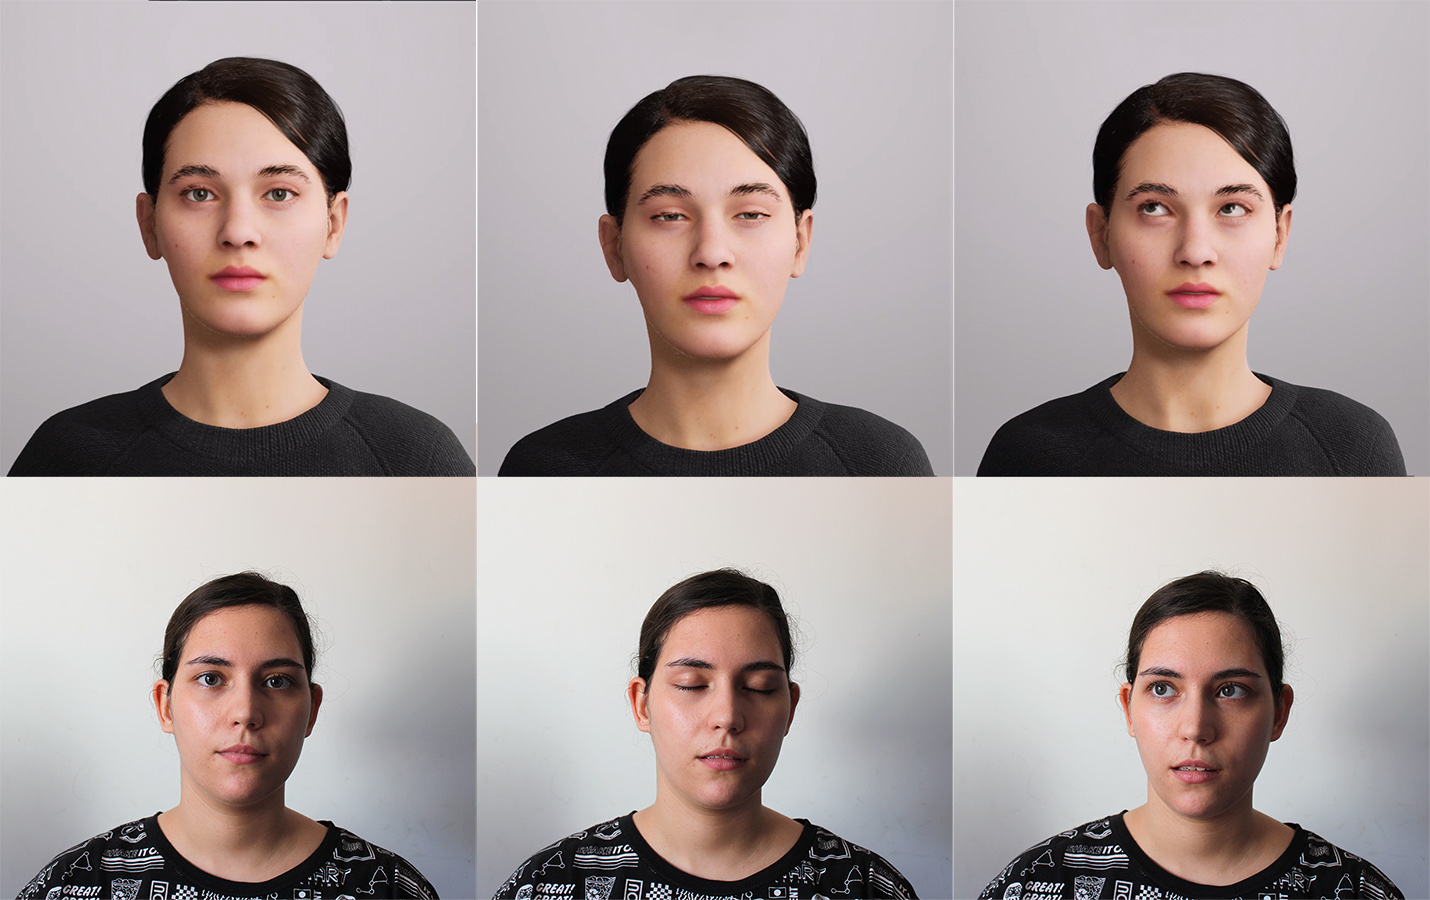
\includegraphics[width=\textwidth]{figures/personavatar.jpg}
\centering
\caption{Different expressions in both the custom metahuman and the actor}
\end{figure}

As it was not necessary to use the developed prototype in its entirety for this study, only the communication between the apple device and the Unreal Engine 4 for the metahuman's animation is required. As a result, the use of customized avatars has no effect on performance levels since all that is required to conduct this experiment is the capture of a local video from the UE4 application.

The experiment was accepted by the university's Data Protection Officer and authorized by the Ethics Committee.

\subsubsection{Procedure}

%An online questionnaire was developed by the authors and posted on social media groups to recruit participants.
%Participants who chose to take part in the study (N=48) were first given an informed consent form. An independent samples design was used for this experiment, where participants were asked to ....

Participants were recruited via email and social media groups, and were required to be at least 18 years old. Our final sample consists of 48 college students (23 female and 25 male), aged between 18 and 45 (M=23.9, SD=5.7). 


%Participants will be recruited via email, sent to the general student population from Madeira University, where they will be briefed about the study's broad, general topic.
%The ones who agree to participate in the test will be asked to complete basic demographic questions and a personality questionnaire used to measure their baseline empathy levels prior to the video/transcript stimuli, and each participant will be randomly redirected to one of the three groups of content using \cite{FER19} and later asked some follow-up questions.

To avoid revealing the experiment's true purpose, and thus distorting the results, participants will be asked to answer some general questions about themselves (from the Big Five Inventory) in addition to the Toronto Empathy Questionnaire \cite{SPR03}, and the questionnaire developed to measure participants' empathy levels, as proposed by \cite{ROT19, ZIB19}. 


\subsubsection{Instruments}
On the pre-test (Appendix \ref{fig:pre}), the Toronto Empathy Questionnaire \cite{SPR03} will be utilized as a control variable, consisting of 16 items (e.g., "I become irritated when someone cries", 1=strongly disagree, to 5=strongly agree). To dispel any suspicions regarding the study's genuine goal, five items from the Big Five Inventory \cite{JOH91} will be incorporated into the questionnaire.

The dependent measures' questions will then be answered on a seven-point Likert-type scale (1=totally disagree, 7=totally agree) on the post-test (see Appendix \ref{fig:videoPost} and \ref{fig:transcriptPost}), based on the work of Bailenson et al. \cite{BAI03}.

We will use four questions to assess the video's perceived authenticity and social presence, presenting the statements ("I feel that the person is watching me and is aware of my presence", "The thought that the person is not a real person crosses my mind often", "The person appears to be conscious and alive to me", "I perceive the person as being only a computerized image, not as a real person") with the above-noted Likert-type scale.

Then, empathy will be tested in both video and transcript groups by using items adapted from the Interpersonal Reactivity Index \cite{DAV83} that deal with cognitive and affective empathy. Three items will be used to test cognitive empathy: "I understand what made her get upset", "Her reactions to the situation are understandable", and “I understand her point of view”. Afterwards three items will be used to measure emotional empathy ("I can relate to her problem", "When I see someone in an unfair situation, I feel frustrated", and “I feel that her emotions are genuine”).

Finally, participants can describe what made them empathize with and/or relate to the person in the video/transcript, as well as what they didn't like.

\subsubsection{Participants}
Participants were recruited via email and social media groups, and were required to be at least 18 years old. Our final sample consists of 48 college students (23 female and 25 male), aged between 18 and 45 (M=23.9, SD=5.7). 

All participants were given an informed consent form and were randomly assigned to one of the conditions (i.e., G1, G2 or G3) using \cite{ALLOCATE.MONSTER}. We have also collected participants' baseline empathy levels using the Toronto Empathy Questionnaire \cite{} prior to the stimuli (---OUR--- mean scores for Males= 47.08, SD=5.54; Females=48.65, SD=7.49).

\makebox[\textwidth]{\color{red} * REVER  *} 

This can also be called Sample. Should have the number of participants, how they were recruited, mean age and standard deviation, how many males/females, etc. and if there was any inclusion and exclusion criteria.
You can also say here that they all were briefed about the study's goal and asked to sign an informed consent form. [If we had given them something for their time, like vouchers etc you should also write this here.]

\subsubsection{Statistical Analysis}
The retrieved data was analyzed in the IBM SPSS statistics software, using a statistical significance level of 0.05.
A Kruskal-Wallis H test was used for ordinal, nonparametric data to assess whether there were any statistically significant differences between the 3 conditions in terms of cognitive and affective empathy. A Mann-Whitney U test was also performed to compare if there were differences in social presence between the metahuman and the real person video conditions.

\subsubsection{Results}
To evaluate the differences in cognitive and affective empathy across conditions, we performed a Kruskal-Wallis test. The test showed no statistically significant differences in cognitive (H(2)=4.30, p=.116) or affective empathy (H(2)=.618, p=.734) for the 3 conditions (metahuman, n=23; real person, n=12; transcript, n=14).

\makebox[\textwidth]{\color{red} * melhorar e dizer pq é bom na discussao E VER H3 *} 

This supports our H1, that CE is the same for all conditions. However, H2... since there is no statistically significant differences in affective empathy...

To assess the difference in social presence between the two video conditions, a Mann-Whitney U test was also performed. The test revealed no significant differences in social presence between the metahuman video (Median=5, n=23) and the real person video (Median=5, n=12), U=121.500, z=-.192, p=.856, r=.004.

\subsubsection{Discussion}